\resizebox{\linewidth}{!}{%
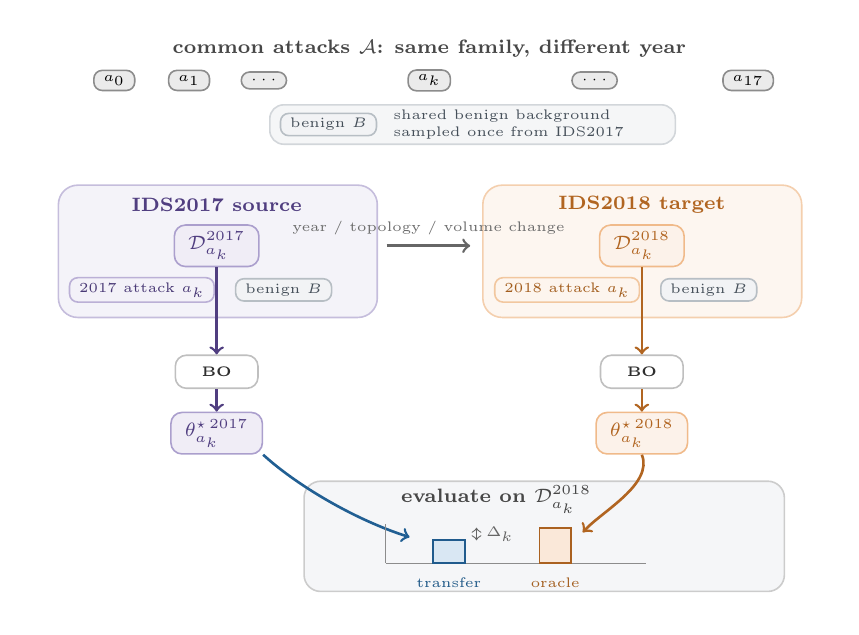
\begin{tikzpicture}[font=\sffamily\scriptsize,line width=0.58pt]
    \definecolor{sourceviolet}{RGB}{103,80,164}
    \definecolor{targetorange}{RGB}{227,130,42}
    \definecolor{transferblue}{RGB}{42,122,188}
    \definecolor{benigngray}{RGB}{96,110,124}
    \definecolor{softgray}{RGB}{245,246,248}

    \tikzset{
        panel/.style={rounded corners=7pt,draw=#1!38,fill=#1!7,inner sep=0pt},
        chip/.style={rounded corners=4pt,draw=#1!55,fill=#1!10,inner xsep=5pt,inner ysep=2.5pt,font=\bfseries\scriptsize,text=#1!78!black},
        smallchip/.style={rounded corners=3pt,draw=#1!45,fill=#1!8,inner xsep=3.5pt,inner ysep=1.8pt,font=\tiny,text=#1!72!black},
        arrow/.style={->,draw=#1!78!black,line width=0.95pt},
        every node/.style={text=black!82}
    }

    \path[use as bounding box] (0,0) rectangle (10.20,7.35);

    % Step 1: choose one attack common to both years and the shared benign background.
    \visible<1->{
        \node[font=\bfseries\scriptsize,text=black!72] at (5.10,7.08)
            {common attacks \(\mathcal{A}\): same family, different year};
        \foreach \x/\lab in {1.10/$a_0$,2.05/$a_1$,3.00/$\cdots$,7.20/$\cdots$,9.15/$a_{17}$}{
            \node[smallchip=black] at (\x,6.68) {\lab};
        }
        \node[smallchip=black] at (5.10,6.68) {$a_k$};

        \node[draw=benigngray!28,fill=benigngray!6,rounded corners=5pt,minimum width=5.15cm,minimum height=0.50cm]
            at (5.65,6.12) {};
        \node[smallchip=benigngray] at (3.82,6.12) {benign \(B\)};
        \node[align=left,font=\tiny,text=benigngray!72!black,anchor=west]
            at (4.52,6.12) {shared benign background\\sampled once from IDS2017};
    }

    % Step 2: build paired datasets for the selected attack.
    \visible<2->{
        \node[panel=sourceviolet,minimum width=4.05cm,minimum height=1.68cm,anchor=north west] at (0.38,5.36) {};
        \node[panel=targetorange,minimum width=4.05cm,minimum height=1.68cm,anchor=north west] at (5.77,5.36) {};

        \node[font=\bfseries\scriptsize,text=sourceviolet!78!black] at (2.40,5.10) {IDS2017 source};
        \node[font=\bfseries\scriptsize,text=targetorange!78!black] at (7.80,5.10) {IDS2018 target};

        \node[chip=sourceviolet] (d17) at (2.40,4.58) {$\mathcal{D}^{2017}_{a_k}$};
        \node[chip=targetorange] (d18) at (7.80,4.58) {$\mathcal{D}^{2018}_{a_k}$};

        \node[smallchip=sourceviolet] at (1.45,4.02) {2017 attack \(a_k\)};
        \node[smallchip=benigngray] (b17) at (3.25,4.02) {benign \(B\)};
        \node[smallchip=targetorange] at (6.85,4.02) {2018 attack \(a_k\)};
        \node[smallchip=benigngray] (b18) at (8.65,4.02) {benign \(B\)};

        \draw[->,draw=black!60,line width=0.95pt] (4.56,4.58) -- node[above,font=\tiny,text=black!58] {year / topology / volume change} (5.62,4.58);
    }

    % Step 3: optimize both year-specific datasets.
    \visible<3->{
        \node[draw=black!25,fill=white,rounded corners=4pt,minimum width=1.05cm,minimum height=0.42cm,font=\bfseries\tiny] (bo17) at (2.40,2.98) {BO};
        \node[draw=black!25,fill=white,rounded corners=4pt,minimum width=1.05cm,minimum height=0.42cm,font=\bfseries\tiny] (bo18) at (7.80,2.98) {BO};
        \draw[arrow=sourceviolet] (d17.south) -- (bo17.north);
        \draw[arrow=targetorange] (d18.south) -- (bo18.north);

        \node[chip=sourceviolet] (theta17) at (2.40,2.20) {$\theta^{\star\,2017}_{a_k}$};
        \node[chip=targetorange] (theta18) at (7.80,2.20) {$\theta^{\star\,2018}_{a_k}$};
        \draw[arrow=sourceviolet] (bo17.south) -- (theta17.north);
        \draw[arrow=targetorange] (bo18.south) -- (theta18.north);
    }

    % Step 4: evaluate both configurations on IDS2018 and compare.
    \visible<4->{
        \node[draw=black!20,fill=softgray,rounded corners=6pt,minimum width=6.10cm,minimum height=1.40cm,anchor=south west] at (3.50,0.18) {};
        \node[font=\bfseries\scriptsize,text=black!72] at (5.95,1.36) {evaluate on \(\mathcal{D}^{2018}_{a_k}\)};

        \draw[arrow=transferblue] (theta17.south east) .. controls (3.40,1.55) and (4.15,1.10) .. (4.85,0.88);
        \draw[arrow=targetorange] (theta18.south) .. controls (7.95,1.55) and (7.28,1.20) .. (7.05,0.94);

        \draw[draw=black!45,line width=0.35pt] (4.55,0.55) -- (7.85,0.55);
        \draw[draw=black!45,line width=0.35pt] (4.55,0.55) -- (4.55,1.05);
        \draw[draw=transferblue!75!black,fill=transferblue!18,line width=0.65pt] (5.15,0.55) rectangle (5.55,0.84);
        \draw[draw=targetorange!75!black,fill=targetorange!18,line width=0.65pt] (6.50,0.55) rectangle (6.90,1.00);
        \node[font=\tiny,text=transferblue!72!black] at (5.35,0.30) {transfer};
        \node[font=\tiny,text=targetorange!72!black] at (6.70,0.30) {oracle};
        \draw[<->,draw=black!60,line width=0.40pt] (5.70,0.84) -- node[right,font=\tiny,text=black!60] {$\Delta_k$} (5.70,1.00);
    }
\end{tikzpicture}%
}
